%*****************************************
\chapter{Grundlagen}\label{ch:preliminaries}
%*****************************************

Wissen, Information, Daten (Winter)
FScore, Precision, Recall
Question Answering (Aggregation, erst FScore für Frage, dann Durchschnitt, oder andersrum)
API, Overfitting


\section*{Inhalte des Kapitels}
- Taxonomie von Ammus (\citet{ammus})
- Transformer Architektur (\citet{attention})

- Neuronales Netz (https://katalog.ub.uni-leipzig.de/Record/0-1066754535)
- Activation Functions (https://katalog.ub.uni-leipzig.de/Record/0-1066754535)
- Backpropagation (https://katalog.ub.uni-leipzig.de/Record/0-1066754535)
- Training eines Modells
    - Batching
    - Optimizer
    - Learning Rate

- Feed-Forward Netze
- Multi-Head Attention
- Encoder und Decoder

- Input embeddings = Embeddings
- Positional Embeddings
- Tokenization
    - Byte Pair Encoding


Sprachmodell Definition (Was ist das)

- Autoregressive Modelle
    - Self-supervised Learning
    - Pretraining
    - continual Pretraining
    - Decoder-Based
    - ZeroShot / FewShot

- Weiterentwicklungen
    - Deep Residual Connections
    - DropOut


\section{Neuronale Netzwerke}
Erstmalig erklärt in \dots

Ein Neuronales Netz besteht aus einer Kombination aus Gleichungen.
Jedes Neuronale Netzt besitzt eine feste Anzahl an Eingabewerten und eine feste Anzahl an Ausgabewerten.
Diese Werte werden folgend als Neuronen $E_N$ und $A_N$ bezeichnet.
$A_N$ berechnet sich aus einer Ansammlung an mathematischen Gleichungen, welche sich ultimativ aus  $E_N$ zusammensetzen.
Neben $A_N$ und $E_N$ besteht ein Neuronales Netz auch aus sogenannten \enquote{Hidden States}, hier als $H_N$ bezeichnet.
$H_N$ agieren sowohl als Ausgabe von vorangegangen Gleichungen, als auch als Eingabe für zukünftige Gleichungen.\\
\begin{figure}
    \centering
    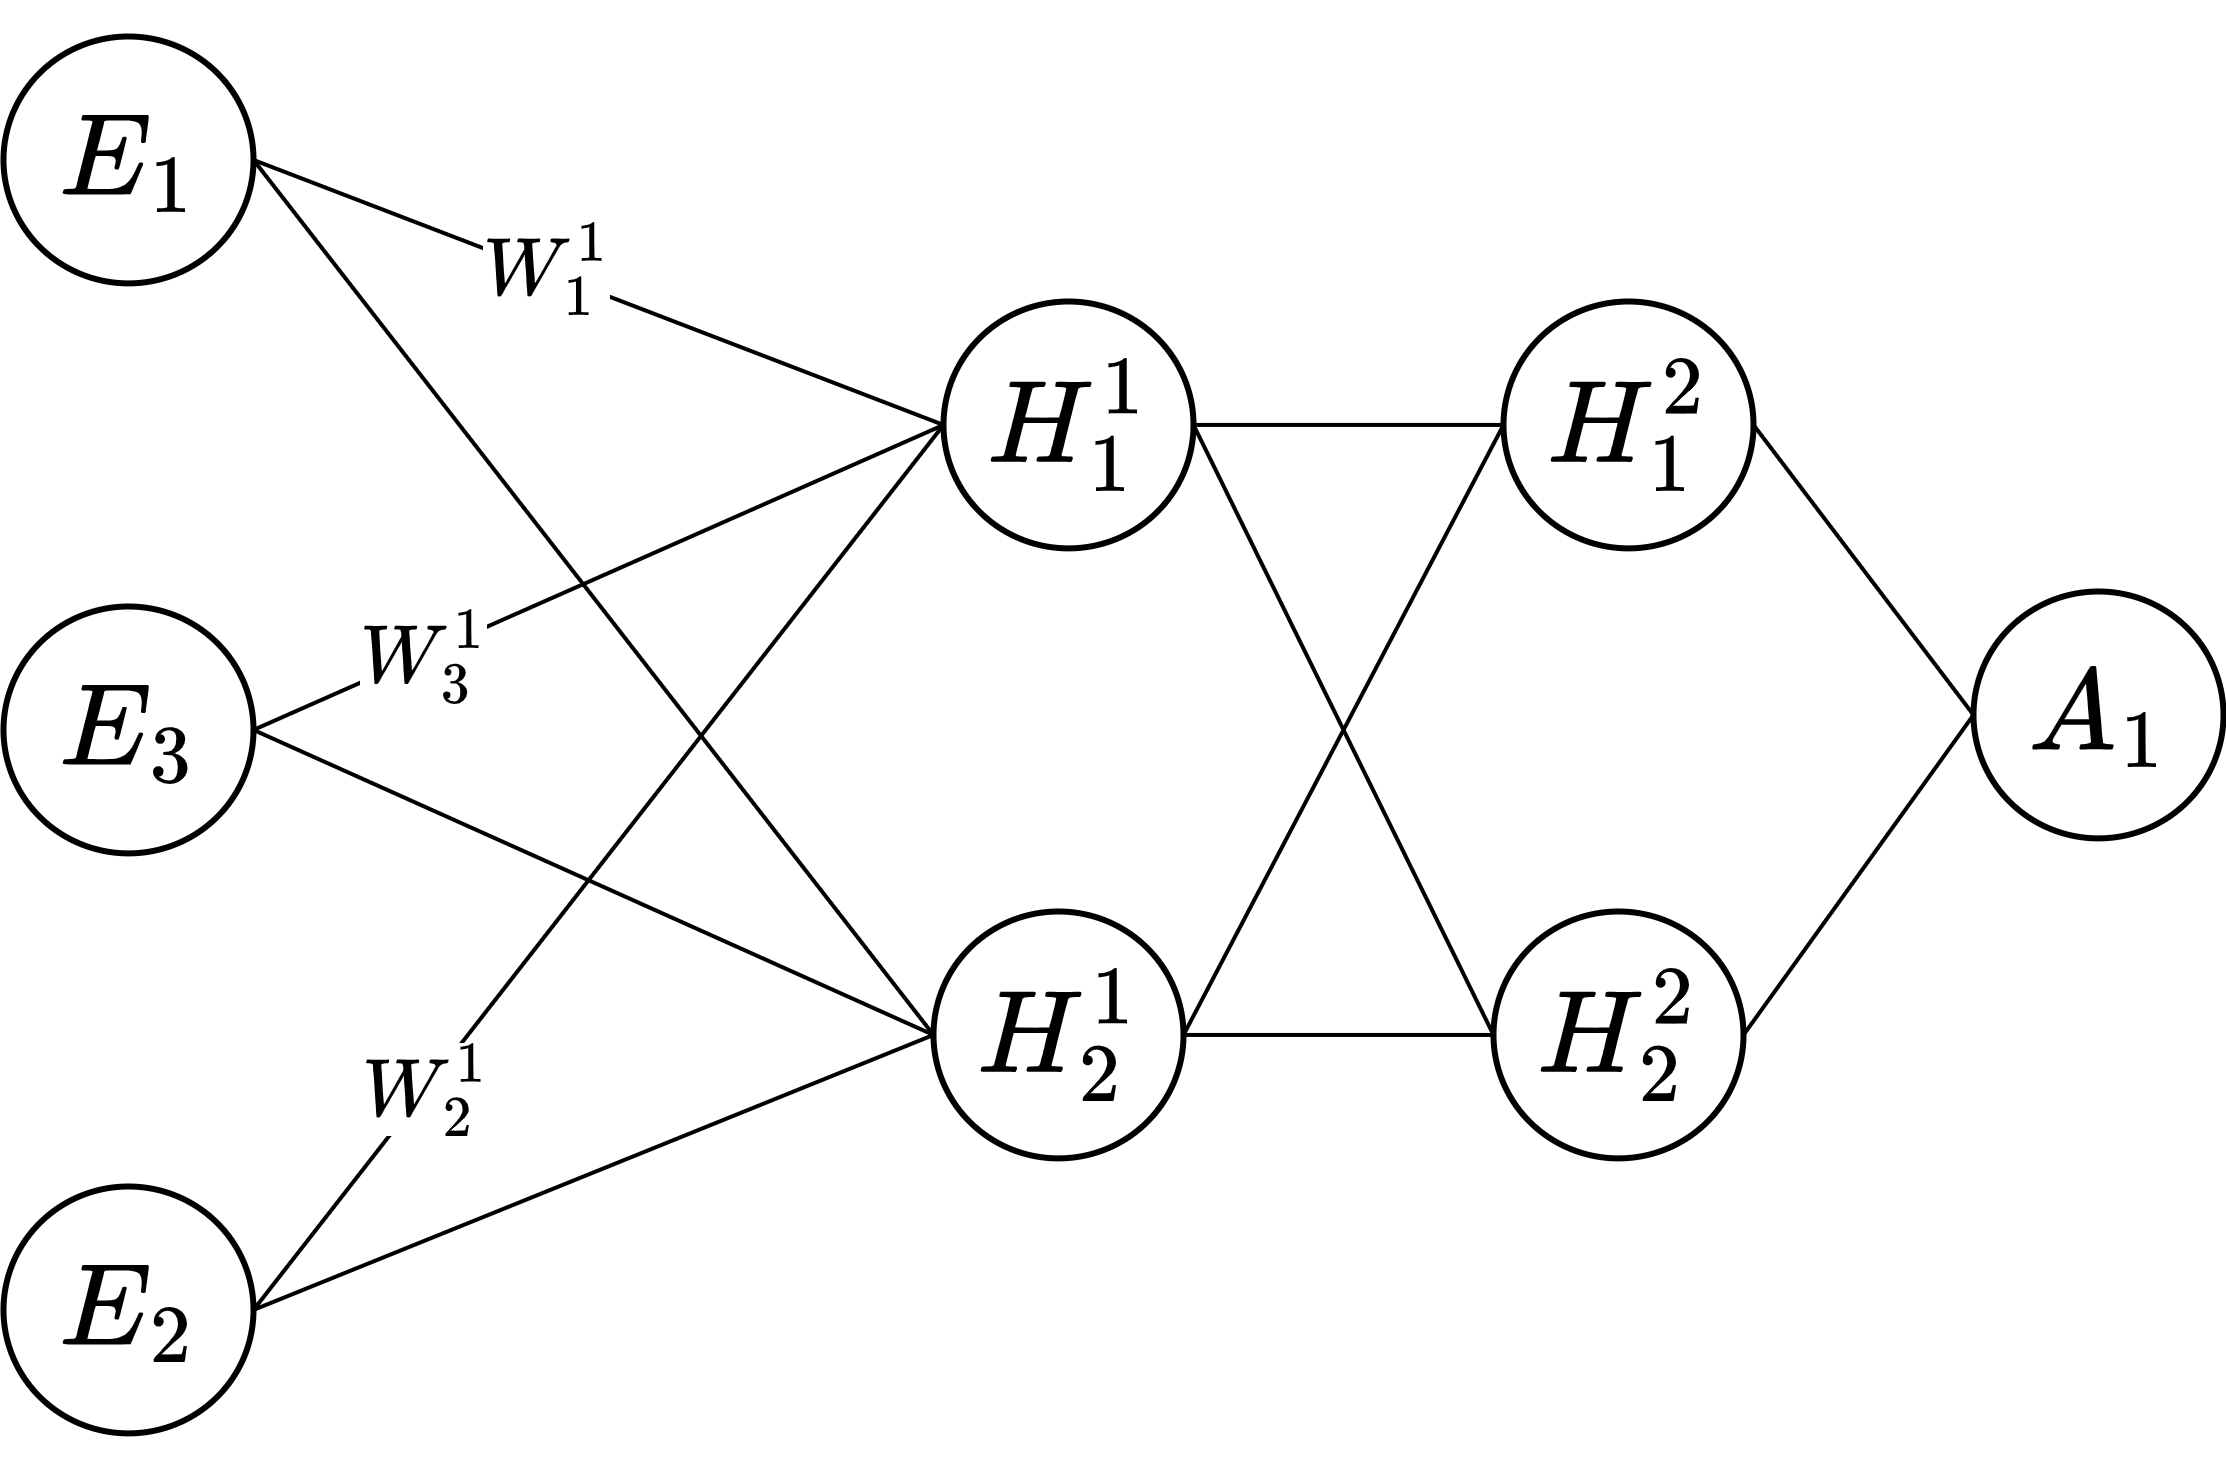
\includegraphics[width=\textwidth]{zeichnungen/nn.png}
    \caption{Beispiel-Aufbau eines Neuronalen Netzes mit 3 Eingabeneuronen, 4 Hidden Neuronen und einem Ausgabeneuron.}\label{nn_simple}
\end{figure}
Abbildung~\ref{nn_simple} zeigt einen Beispielaufbau mit 3 $E_N$, hier bezeichnet als $E_1,E_2,E_3$, zwei Hidden Layer mit je zwei $H_N$, hier bezeichnet als $H^1_1, H^1_2$ und $H^2_1, H^2_2$ und einem Ausgabeneuron $A_1$.
Bei der Nutzung dieses Neuronalen Netzes wird von der Eingabe zur Ausgabe gerechnet.
Dies bedeutet $E_N$ ist gegeben, und zu erst werden $H^1_N$ berechnet.
Eine Beispielgleichung für $H^1_1$ ist wie folgt:
\begin{align}
    H^1_1=ReLU(W^1_1*E_1 + W^1_2*E_2 + W^1_3*E_3 + B^1_1)
\end{align}
$W^1_N$ repräsentiert hier sogenannte Gewichte.
Gewichte sind Parameter, die während des Trainings eines Netzwerkes angepasst werden, um eine optimale Ausgabe von $A_N$ zu erhalten.
Diese Parameter nennt man auch lernbare Parameter.
$B^1_N$ ist der Bias und ist ebenso ein lernbarer Parameter.
Alle Werte der Eingabe werden der Formel folgend zusammengerechnet und mit Hilfe einer Aktivierungsfunktion umgewandelt.
Diese Aktivierungsfunktion war in früheren Netzen die Sigmoid-Funktion mit $f(x)=\frac{1}{1+e^{-x}}$.
In modernen Netzen und ebenso in Transformer-Modellen wird hier die ReLU Funktion verwendet, welche als $f(x)=max(0,x)$ definiert ist.
Beide Funktionen sind in Abbildung~\ref{activation_functions} dargestellt.
Üblicherweise repräsentiert eine Aktivierungsfunktion eine Transformation der Eingabewerte auf einen Non-linearen Ausgabewert zwischen 0 und 1.
Jedoch ist dies nicht zwingend notwendig, da zum Beispiel die ReLU Funktion nur Werte zwischen 0 und $\infty$ ausgibt, sich jedoch schneller berechnen lässt als die Sigmoid-Funktion.
Aktivierungsfunktion sind notwendig, um die Komplexität eines Neuronalen Netzes zu erhöhen und damit die Fähigkeit, komplexere Probleme zu lösen, zu ermöglichen.
Ohne eine Aktivierungsfunktion würden $A_N$ Neuronen eine Linearkombination der Eingabewerte ergeben, wodurch hier nur lineare Probleme gelöst werden können.
Ein einfaches Beispiel wäre die Berechnung der XOR-Funktion. Die XOR-Funktion verbindet zwei Eingaben und ergibt eine Ausgabe, ist eine der beiden Eingaben 1, soll die Ausgabe ebenso 1 sein.
Andernfalls soll die Ausgabe 0 sein. Diese einfache Funktion kann nicht ohne eine Aktivierungsfunktion gelöst werden.\\

\begin{figure}
    \centering
    \begin{minipage}{0.45\textwidth}
        \centering
        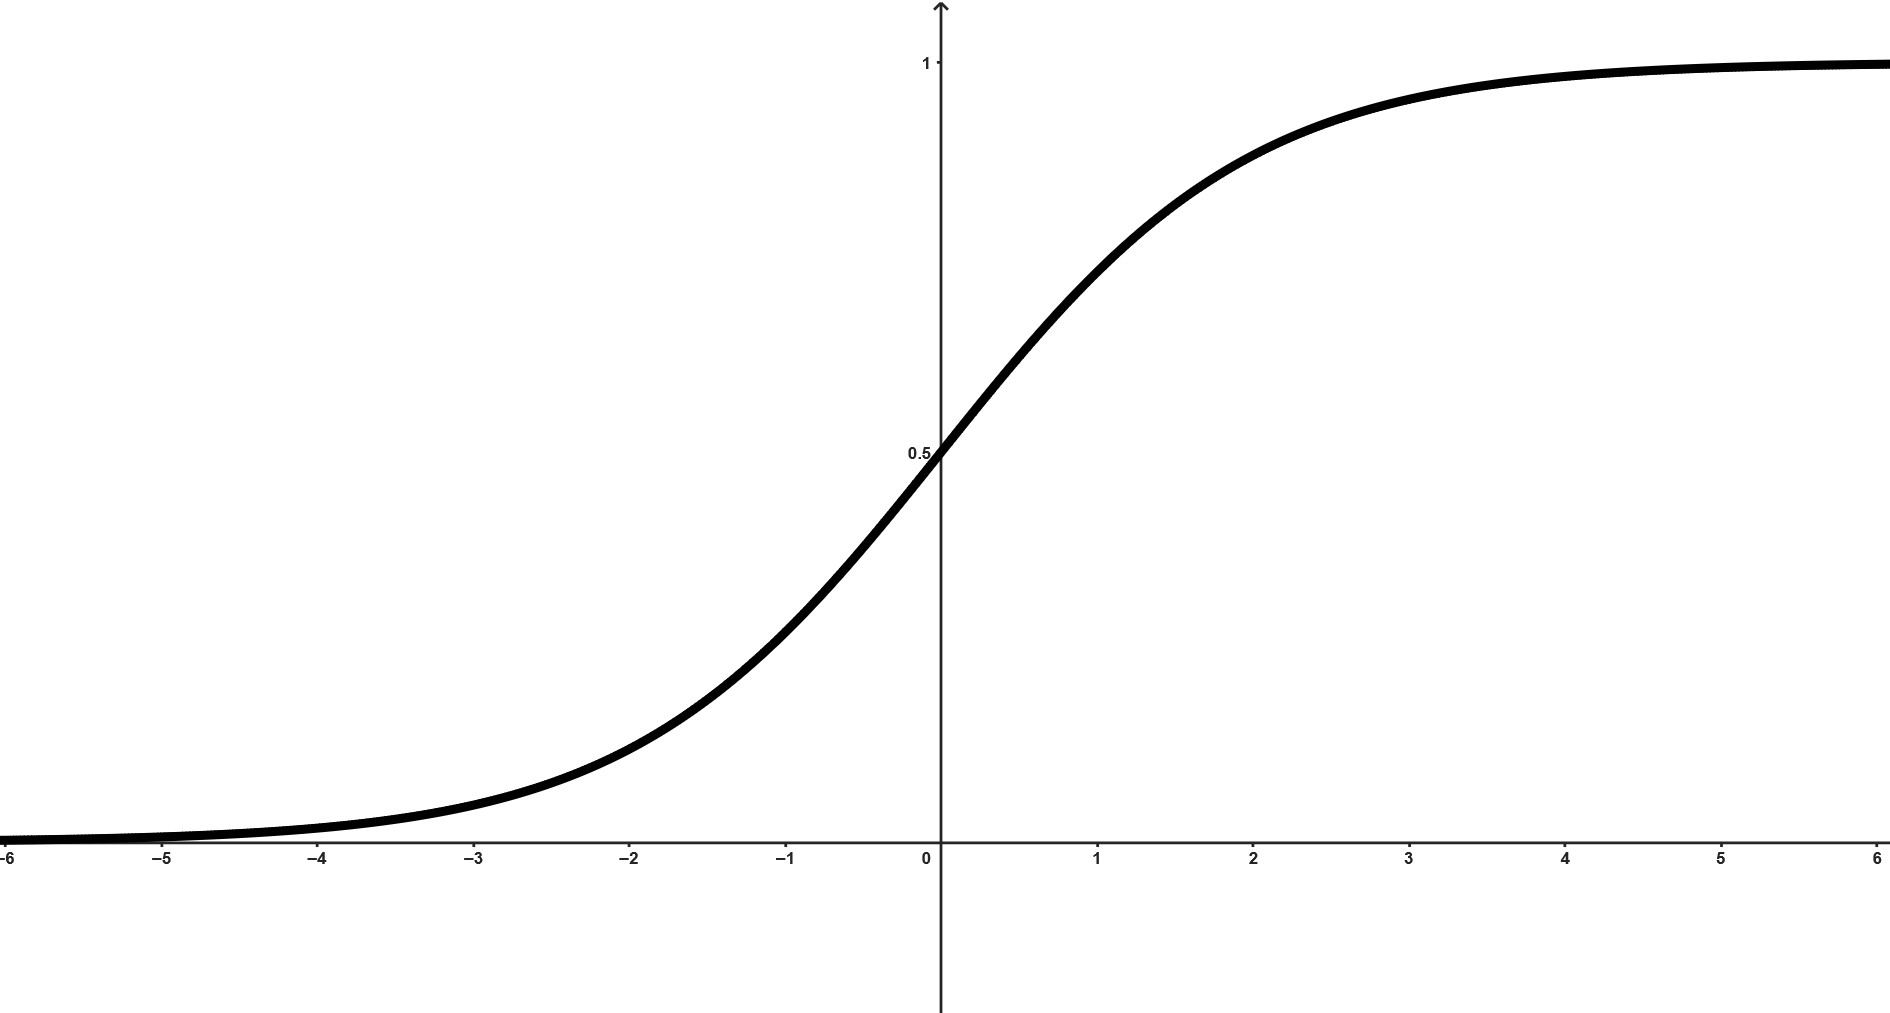
\includegraphics[width=0.9\textwidth]{zeichnungen/sigmoid.png}
        \caption*{Die Sigmoid-Funktion}
    \end{minipage}\hfill
    \begin{minipage}{0.45\textwidth}
        \centering
        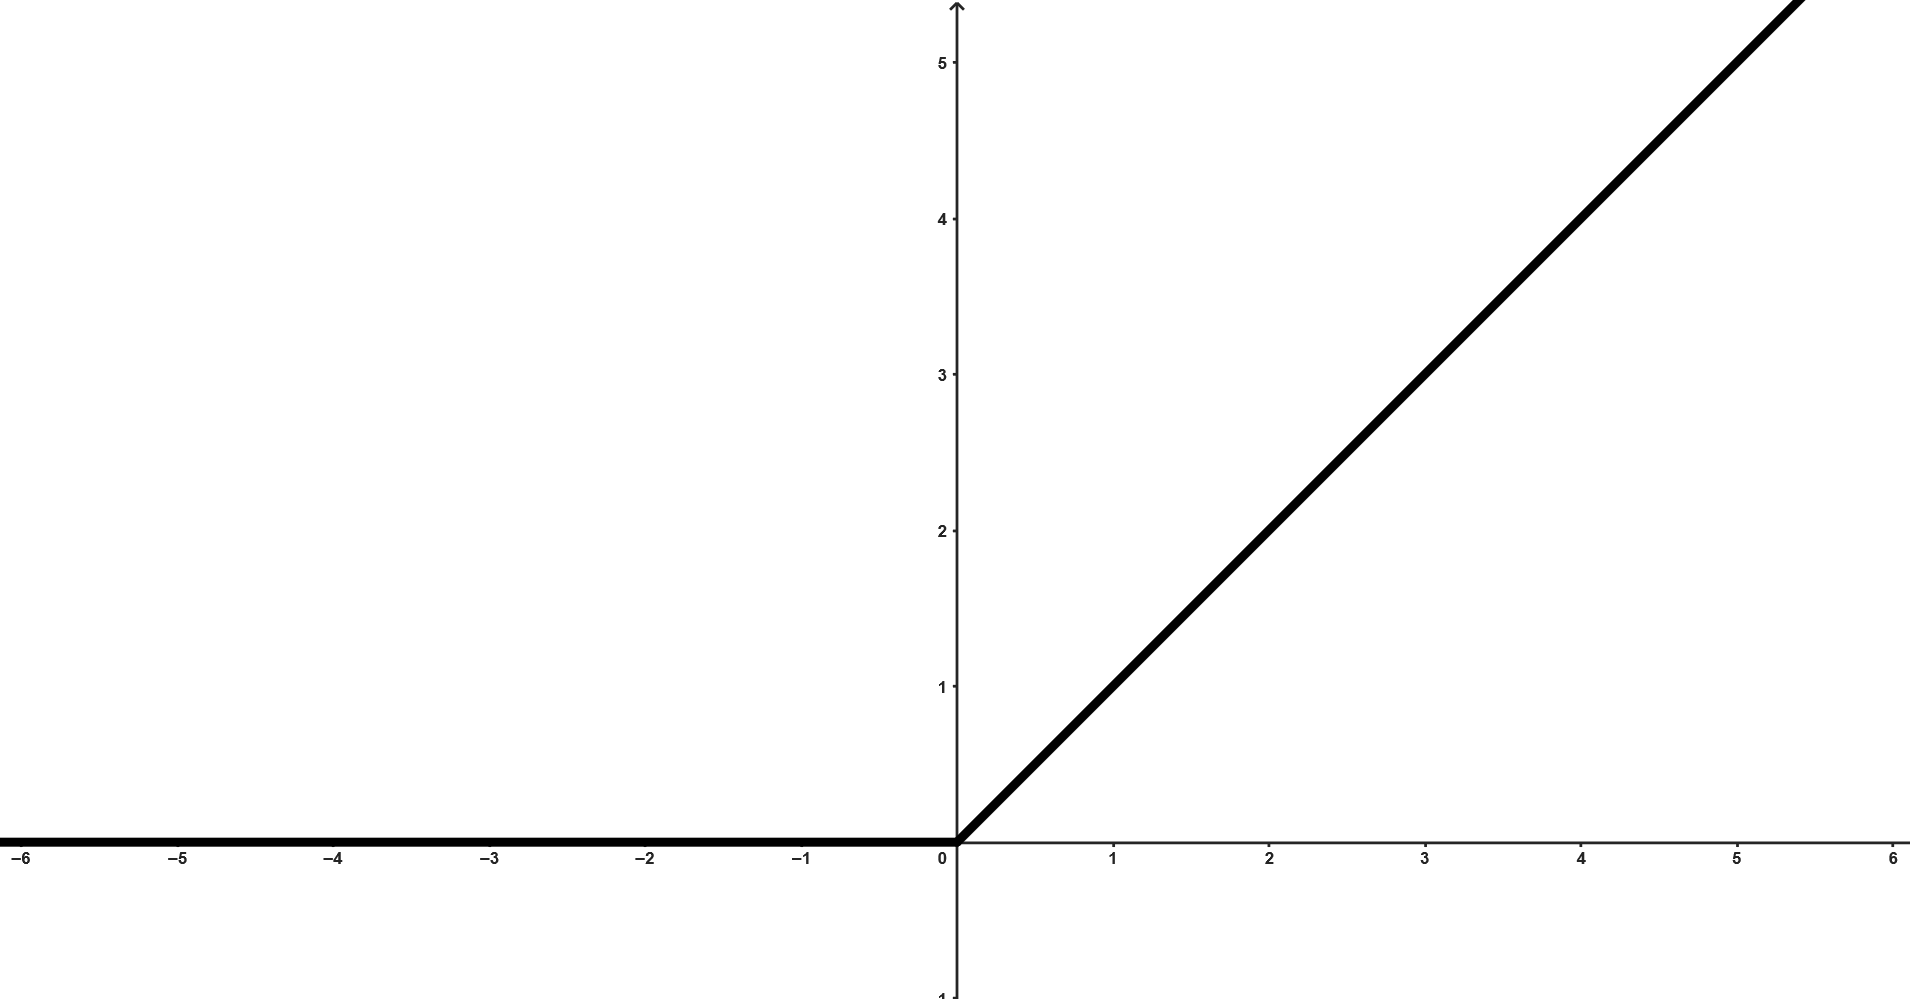
\includegraphics[width=0.9\textwidth]{zeichnungen/relu.png}
        \caption*{Die ReLU-Funktion}
    \end{minipage}
    \caption{Aktivierungsfunktionen von Neuronalen Netzen.}\label{activation_functions}
\end{figure}

Die Ausgabe $A_N$ sind ebenso Werte in dem Bereich der Aktivierungsfunktion und sind nicht immer repräsentativ für das Problem, das das Neuronale Netz lösen soll.
Deshalb werden diese Werte interpretiert und repräsentieren häufig einen Confidence-Score für eine bestimmte Klasse.
Ist das Neuron $A_1$ auf dem Maximalwert 1, dann ist das Netz zu 100\% sicher, dass die Eingabe der Klasse 1 enspricht.
Im Bezug auf Transformer ist die Ausgabe $A_N$ ein Vektor über das gesamte Vokabular des Transformers, und gibt aus, in wie fern das Modell glaubt, das jeweilige Token folgt auf den Eingabetext.\\

Mit Hilfe dieser Ausgabe kann nun eine Kostfunktion beschrieben werden.
Eine Kostfunktion ist eine Funktion, welche angibt, wie falsch das Modell liegt.
Bei einem Neuronalen Netz, welches Klassifiziert, wäre eine einfache Kost-Funktion die Summe der Differenzen zwischen der Ausgabe des Netzes und der tatsächlichen Klasse.
Je kleiner die Kost-Funktion, desto näher ist das Modell an der eigentlichen Ausgabe.
Hier existiert auch bereits die Unterscheidung zwischen einem Überwachten, Selbstüberwachten und Unüberwachten Lernverfahren.
Bei einem Überwachten Lernverfahren sind die gewollten Ausgabeneuronen bekannt und können mit der Ausgabe des Modells verglichen werden.
Dies vereinfacht die Kost-Funktion.
Selbstüberwachte Lernverfahren nutzen den selben Prozess, jedoch wird hier die Eingabe genutzt, um die Kost-Funktion zu berechnen.
Bei Unüberwachtem Lernen ist die Ausgabe nicht bekannt, sondern wird durch einen separaten Prozess interpretiert.
Ein Beispiel für ein Überwachtes Lernen wäre die Klassifizierung von Bildern.
Der Datensatz enthält sowohl Bilder, als auch zugehörige Klassen.
Somit ist die erwartete Ausgabe des Modells zu einem Bild exakt die Klasse.
Transformer-Modelle sind Selbstüberwachte Systeme.
Hier ergibt sich aus der Eingabe die Erwartete Ausgabe, da der darauf folgende Token der Eingabe als korrekt angesehen wird.
Unüberwachtes Verfahren sind zum Beispiel Agents, welche Spiele lernen.
Hier existiert in den meisten Fällen eine Belohungsfunktion, welche angibt, wie gut das Modell gespielt hat.
Belohungsfunktionen können beschreiben, wie weit das Auto im Spiel gefahren ist oder wie viele Punkte gesammelt wurden.\\

\section{Transformer}\label{sec:transformer}
%\todo{
%Grundlagen:
%- das was du schon drin hast mit "General Pretrained Transformer - Neuronal Networks - Zero Shot Ansatz - Finetuning - Datenkuration"
%- aber alles was mit GPT zu tun hat nicht, das ist ein spezieller Ansatz und das sollte zu state of the art
%- alles was im Titel steht :-) Question Answering, unsupervised und supervised training und so
%- Definitionen Daten, Informationen und Wissen nach Winter passt hier denke ich auch rein
%
%State of the Art:
%- aktuelle Paper
%- Vergleich verschiedener Systeme und Modelle
%- und das was du da schon hast, also das meiste ist ja schon am richtigen Ort
%}
Die erste schriftliche Erwähnung des Transformer-Modells und zusätzlich auch die Einführung der beiden Teilmodelle Encoder und Decoder findet sich in \citet{attention}.
Die hier beschriebene bidirektionale Architektur bildet die Grundlage für alle darauf aufbauenden Modelle und Weiterentwicklungen.
Die grundlegende Architektur wurde für verschiedene Anwendungen stark modifiziert.
Seit 2017 gibt es grundlegende Unterschiede in den Modellen und deren Möglichkeiten.
Aus diesem Grund haben \citet{ammus} eine Taxonomie der Transformer-basierten vortrainierten Sprachmodelle eingeführt.
Diese Taxonomie wird hier zur Beschreibung weiterer Architekturen und Methodiken verwendet.\\

Neben dem Grundbaustein eines Transformers - dem Attention-\ac{nn} - sind zwei wichtige Modifikationen gegenüber normalen neuronalen Netzen in Transformer eingeflossen.
Residuale Verbindungen als Level-Normalisierung, auf Englisch \enquote{Deep Residual Connections}, verändern das Ziel eines \ac{nn}, behalten aber durch ihre Level-Normalisierung die gleichen Ausgaben bei.
Dieses Konzept wurde erstmals in \citet{deep_residual} eingeführt und liefert die Lösung für ein grundlegendes Problem von großen, aus mehreren Ebenen bestehenden Transformer-Modellen.
Bereits 2016 wurde im Bereich der Bilderkennung festgestellt, dass sich die Korrektheit von Modellen mit zunehmender Tiefe sättigt und dann schnell verschlechtert, wenn dieses Modell weiter trainiert wird.
Dies setzte eine praktische Grenze für die Tiefe von \ac{nn}s und verhinderte somit die Lösung komplexerer Probleme mit größeren Modellen.
\citet{deep_residual} beschreiben eine Lösung durch die genannten Residuen, die normale \ac{nn} simple ersetzen können, und zeigen ebenfalls die Wirksamkeit dieser Methode.\\

Die zweite wichtige Änderung ist die Einführung von Dropout.
Dropout ist eine Methode, die die Trainingszeit von \ac{nn}s verkürzt und die Generalisierung verbessert.
\citet{dropout} beschreiben die Methode als das zufällige Aussetzen von Neuronen in einem \ac{nn}. 
Diese Aussetzung hängt nicht von der Eingabe ab.
Durch das Aussetzen von Neuronen wird das \ac{nn} gezwungen, sich nicht auf andere Neuronen zu verlassen und somit eine bessere Generalisierung zu erreichen.
Das Aussetzen erfolgt nur während des Trainings und nicht während der Inferenz.
Die Methode wurde 2014 eingeführt und ist seitdem ein fester Bestandteil von \ac{nn}s.\\

\section{Tokenization}\label{sec:tokenization}
Transformer-Modelle können Eingaben nicht ohne zusätzliche Umwandlung verarbeiten.
Neben der Erzeugung von Kodierungsvektoren muss die Eingabe zunächst in kleinere Einheiten, sogenannte Tokens, zerlegt werden.
Verschiedene ältere Modelle verwenden dazu Wörter oder Symbolunterteilungen.
Dies ist jedoch problematisch.\\

Durch die Zerlegung der Eingaben in Symbole ist zwar das Vokabular kleiner, welches zu schnelleren Trainingsdurchläufen führt, jedoch muss das Modell vor dem Erlernen von Wortzusammenhängen, Satzstrukturen und Sachverhalten zunächst die Bedeutung der Wörter und deren Zusammensetzung aus Symbolen erlernen.
Dies führt dazu, dass ein großer Teil der Trainingszeit für das Erlernen der Sprache verloren geht, was die endgültige Leistungsfähigkeit der Modelle massiv einschränkt \citep{bpe}.
Eine logische Schlussfolgerung wäre hier die Verwendung von Wörtern oder sogar Satzphrasen als Tokens.
Mit zunehmender Größe der Datensätze, die zum Training der Modelle verwendet werden, wächst hier das Vokabular immens an.
Dies führt zu einer starken Verlangsamung der Trainingsläufe und zu sehr großen Modellen ohne Vorteil in ihrer Leistungsfähigkeit.
Wörter mit gleichem Wortstamm oder ähnlicher Bedeutung aufgrund grammatikalischer Regeln (Plural, Genus, Tempora) müssen vom Modell erst als \enquote{gleiches Wort} gelernt werden.
Daher hat sich die Unterteilung von Wörtern in Teilwörter als Standard durchgesetzt.

\subsection{Byte-Pair-Encoding}\label{subsec:bpe}
\citet{bpe} schlugen zu diesem Zweck die Verwendung von \ac{bpe} vor.
Die Unterteilung von Wörtern in Untergruppen von Wörtern hat bereits bei der Übersetzung von Sätzen zu erheblichen Verbesserungen geführt.
Sie hat sich aber auch in anderen Bereichen und Aufgaben wie der Textgenerierung, der Textklassifikation und der Analyse von Emotionen durchgesetzt.
Die Unterteilung von Wörtern ist hier eher als das Zusammenfügen kleinerer Teilwörter zu verstehen.
Ausgehend von einem Vokabular, das aus allen Symbolen eines Alphabets besteht, wird dieses durch das Zusammenführen (engl.
\enquote{Merge}) von Symbolen erweitert, deren Kombination im Datensatz am häufigsten vorkommt.
Dieser Vorgang wird solange wiederholt, bis die gewünschte Anzahl von Teilwörtern erreicht ist.
Die Anzahl der Teilwörter ist dabei ein Hyperparameter, der je nach Modell und Datensatz variiert.\\

Die Unterteilung von Wörtern in Teilwörter hat den Vorteil, dass die Größe des Vokabulars nicht mit der Größe des Datensatzes wächst.
Dies führt zu einer schnelleren Eingabeverarbeitung und einer besseren Generalisierung der Modelle.
Die Unterteilung von Wörtern in Teilwörter hat jedoch auch Nachteile.
Sie ist nicht eindeutig, d.h.
ein Wort kann in unterschiedliche Mengen von Teilwörtern zerlegt werden.
Dies führt zu einer größeren Anzahl möglicher Eingaben, die das Modell lernen muss.
Ein weiterer Nachteil ist, dass die Zerlegung von Wörtern in Teilwörter nicht immer sinnvoll ist.
So kann es vorkommen, dass ein Wort in Teilwörter zerlegt wird, die in der Sprache nicht existieren.
Dies wiederum minimiert die Verallgemeinerbarkeit der Modelle.
Ein Beispiel hierfür ist das Wort \enquote{Datensatz}.
Eine sinnvolle Unterteilung wäre hier \enquote{Daten} und \enquote{satz}, aber durch den Aufbau des Vokabulars aus den Symbolen des Datensatzes kann es vorkommen, dass das Teilwort \enquote{Daten} nicht die notwendige Häufigkeit besitzt und somit nicht im Vokabular vorhanden ist.
Daher muss auch dieses Wort zerlegt werden, z.B.
in \enquote{Da} und \enquote{ten}.
Beide Teilwörter haben in der deutschen Sprache keine Bedeutung, werden aber durch das Modell mit Bedeutung belegt und in Beziehung zu anderen Wörtern gesetzt.
Dies führt zu einer unverständlichen Bedeutungsannotation von Teilwörtern und verschlechtert sowohl die Leistung als auch die Nachvollziehbarkeit des Modells und erschwert die Forschung an den Modellen.


